In dieser Messaufgabe, wurde die primärseitige Spannung mittels eines Stelltransformators variiert. Durch erhöhung dieser Spannung mit Schritten von 40 V, wurde die sekundärseitige Spannung bis der Bemessungswert von $U_{1L} = 400 \text{V}$ erreicht wurde bemessen. Der Strom der bei der Bemessungsspannug auftaucht (auch Leerlaufstrom genannt) einschließlich der Wirkleistung wurden auch bemessen und dokumentiert. \par  
Die Messschaltung für diese Schaltung is in der unteren Abbildung dargestellt. \par 
\begin{figure}[H]
    \centering
    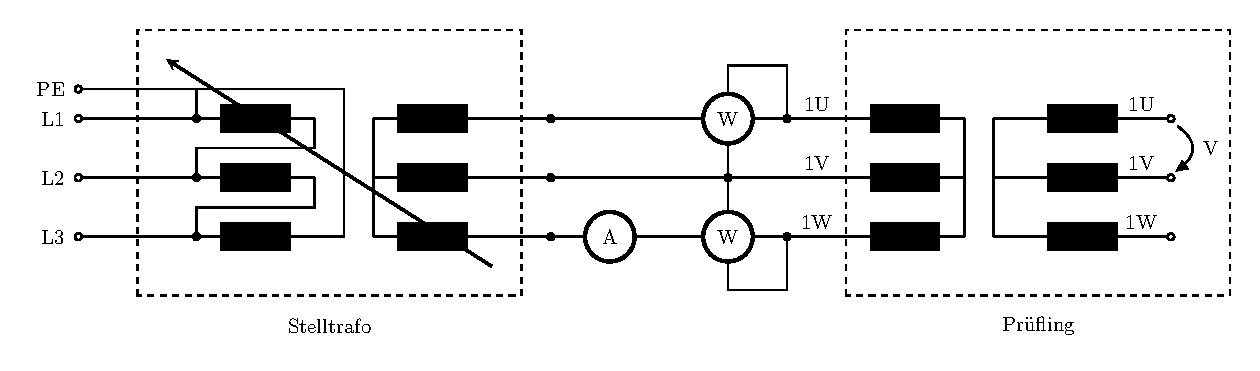
\includegraphics[width=0.95\textwidth]{fig/ll_mess.pdf}
    \caption{Messschaltung Leerlaufversuch }
\end{figure}
 Die Abhängigkeiten $U_{2L} = f(U_{1L}) $ und $ \text{ü} = f(U_{1L})$ sind in den unten stehenden Diagrammen dargestellt.  \par 
% LEERLAUF U_1L vs U_2L
  \begin{figure}[H]
	\begin{subfigure}{0.48\textwidth}
	  \centering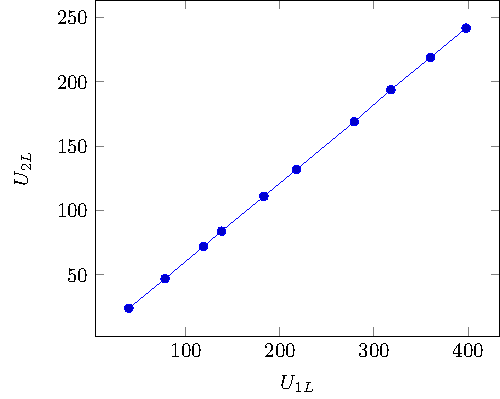
\includegraphics[width=0.95\textwidth]{fig/ll_u1ue.pdf}
	\end{subfigure}
	\begin{subfigure}{0.48\textwidth}
	  \centering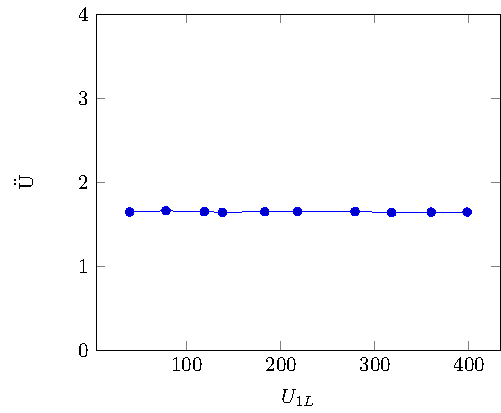
\includegraphics[width=0.95\textwidth]{fig/ll_ue.pdf}
	\end{subfigure}
	\caption{$U_{2L}$ (\si{\volt})  und Übersetzungsverhältnis ü in Abhängigkeit von $U_{1L}$ (\si{\volt})  }
  \end{figure}
  
Zusätzlich wurden die folgenden Werte bei  $U_{1L} = 400 \text{V}$ erhalten: \\
\begin{align*}
  \intertext{Leerlaufstrom: } I_{l} &=  \SI{472.1}{\milli\ampere}  \\  
  \intertext{Wirkleistung: }
 P_l &= P_{UV} + P_{VW}  \\
&=  \SI{-98}{\watt} + \SI{160}{\watt}\\
&=  \SI{62}{\watt}    \\
\intertext{Übersetzungsverhältnis:} \text{ü} &= \frac{U_{1L}}{U_{2L}} \\&= \frac{ \SI{398}{\volt}}{ \SI{241.9}{\volt} } \\
&= 1.65 \\
\intertext{Eisenstrom: } I_{Fe} &=
\frac{P_l}{U_{1L}} \\
&=  \SI{90}{\milli \ampere}  \\
\intertext{Hauptflussstrom: } I_{H} &=
\sqrt{I_{1L}^2-I_{Fe}^2} \\
&=  \SI{463.45}{\milli \ampere}\\
\intertext{Eisenwiderstand: } R_{Fe} &= \frac{U_{1L}}{\sqrt{3}\cdot I_Fe} \\
&= \frac{ \SI{398}{\volt}}{ \SI{90}{\milli\ampere} } \\
&= \SI{2.55}{\kilo\Omega}\\
\intertext{Hauptinduktanz: } X_{h} &= \frac{U_{1L}}{\sqrt{3} \cdot I_{\mu} } \\
&= \frac{ \SI{398}{\volt}}{ \sqrt{3}\cdot \SI{463.45}{\milli\ampere} } \\
&= \SI{0.496}{\kilo \Omega}  \\
\intertext{Leistungsfaktor: } cos(\varphi) &= \frac{\sqrt{3}*P_l}{3*U_{1L}*I_{1L}} \\
&=  0.19
\end{align*}

\begin{figure}[H]
    \centering
    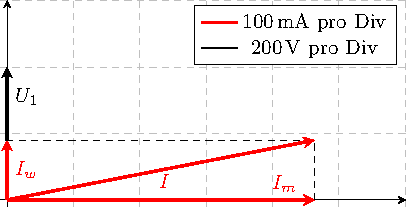
\includegraphics{fig/phasor_open.pdf}
    \caption{Caption}
    \label{fig:open}
\end{figure}